\Chapter{PROSPECT Experiment}
    
    The RAA described in Chapter~\ref{Ch2} leads to the need of an experiment able to probe the short baseline sterile neutrino oscillation, as well as direct measurement of the flux and spectrum of a single fission fuel reactor. 
    The experiment has to meet the requirements of 
    \begin{itemize}
        \item Sub-10~m baseline from a reactor with compact reactor size. 
        \item Fission reactor whose neutrino production is from a single isotope.
        \item High IBD position reconstruction for oscillation measurement.
        \item High energy resolution to precisely measure neutrino spectrum.
    \end{itemize}
    
    PROSPECT~\cite{bib:prospect_physics, bib:prospect_nim}, the Precision Reactor Oscillation and SPECTrum experiment, was designed and built to direct measure neutrino fluxa and spectrum from the High Flux Isotope Reactor (HFIR) located at Oak Ridge National Laboratory (ORNL), USA. 
    PROSPECT's antineutrino detector (AD) covers various baseline from 7~m to 9~m with segmented LS.
    The goal of PROSPECT is to probe the $\sim$1~eV scale sterile neutrino oscillation by the observation of \nuebar disappearance, and precisely measure reactor neutrino spectrum from only $^{235}$U.
    
\Section{HFIR Reactor}

    HFIR reactor is a high enrichment $^{235}$U (HEU) research fission reactor, whose $^{235}$U enrichment is 93\% in average.
    The key parameters of HFIR reactor for PROSPECT neutrino measurement are shown in Table~\ref{tab:HFIR}.
\begin{table}[h]
    \centering
    \begin{tabular}{cc}
    \hline
    \hline
    Parameter  & Value   \\ 
    \hline
    Power    & 85~MW \\
    \hline
    Dimensions     & 435~mm (diameter) $\times$ 508~mm (height) \\
    \hline
    $^{235}$U enrichment & 93\% \\
    \hline
    Neutrino source & $\sim$99\% from $^{235}$U \\
    \hline
    Reactor cycle & $\sim$25~day on, $\sim$30~day off \\
    \hline
    \hline
    \end{tabular}
    \caption[HFIR parameters]{The properties of the HFIR reactor.}
\label{tab:HIFR}
\end{table}

\begin{figure}
    \centering
    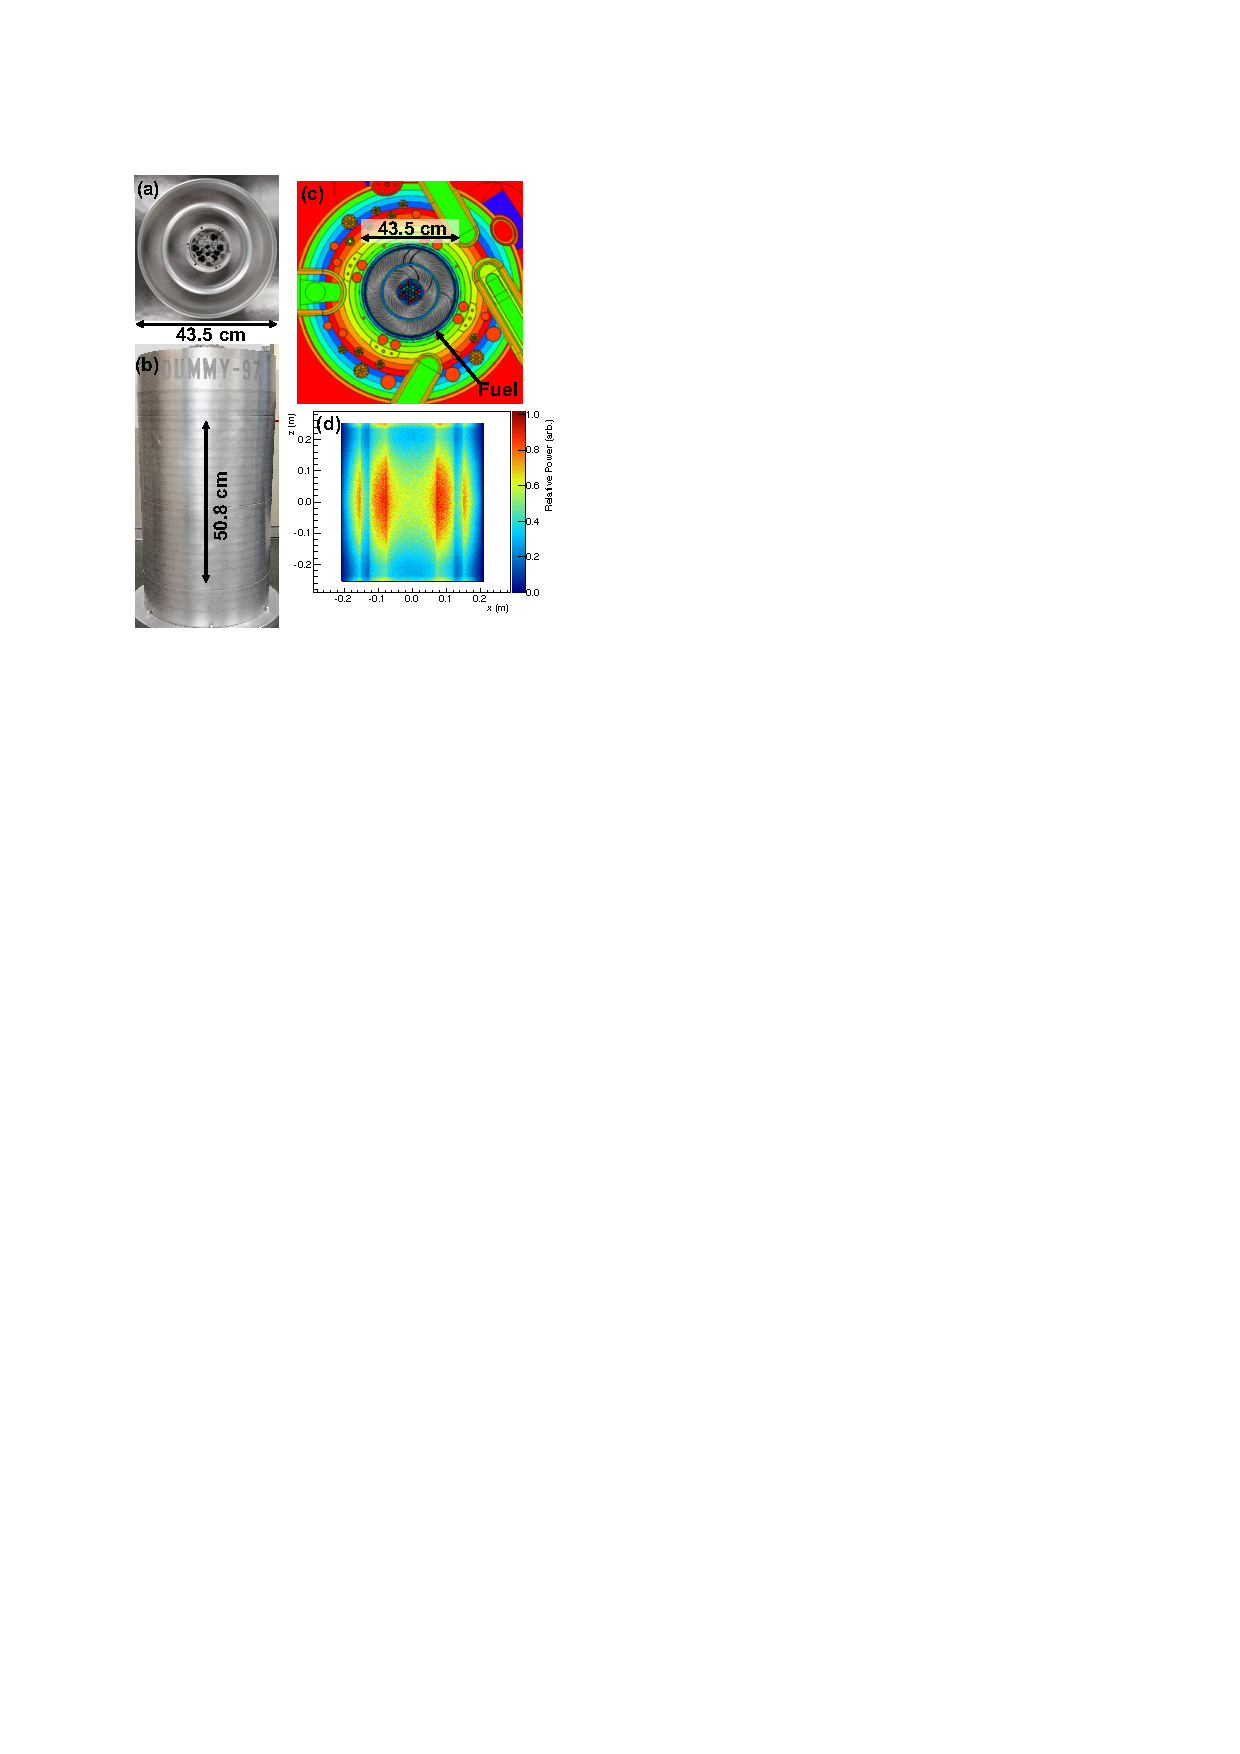
\includegraphics[width=0.5\textwidth]{Figures/HFIR.pdf}
    \caption[The dimensions and power distribution of HFIR]{(a) and (b) the diameter and height of the HFIR core.
    The location of the HFIR core in a detailed reactor system simulation is indicated in (c).
    (d) is a projection of the fission power density of HFIR at the x-z plane.}
    \label{fig:HFIR}
\end{figure}

    The HFIR a cylindrical fission reactor.
    Its compact size, as shown in Table~\ref{tab:HIFR} and Fig.~\ref{fig:HFIR}, is ideal to limit the uncertainty of baseline.
    To maintain its high $^{235}$U enrichment, the HFIR reactor has relatively short reactor cycles.
    In this case, the fuel evolution of fissile isotopes is negligible.
    
    The HFIR facility also brought unique challenge of background for neutrino measurement. 
    Because of the very short baseline requirement of the experiment and availability of the experiment site, the PROSPECT AD is exposed to cosmic ray background with minimal overburden. 
    The detector also faces reactor correlated background, e.g. the neutron background generated from reactor and the $\gamma$ ray background from the metallic materials in the piping of the facility.
    A comprehensive background characterization is therefore organized in the research and development (R\&D) phase of PROSPECT~\cite{bib:prospect_background}. 
    

\Section{Detector Design}

\Section{Antineutrino Detection}

\Section{Optical Grid}

\Section{Detector Construction and Commissioning}

\Section{Data Acquisition}